\documentclass[11pt,a4paper]{article}  % Déclare la classe du document.

\newcommand{\chaptermark}[2]{\og #2 \fg{} (#1)} % ligne uniquement pour éviter une erreur en cas d'article
\include{../1ere-preambule}

\usepackage{epic}   % extension et simplification de  l'environnement picture
\usepackage{graphicx}    % permet d'inclure des graphique externe dans un document
\usepackage{arydshln}   %permet d'avoir des lignes en pointillés

\newcommand{\lignes}[1]{
	\setlength{\unitlength}{1mm}
	\vskip 0,4cm\noindent
	\multido{\i=0+1}{#1}{%
		\noindent
		\begin{picture}(150,5)
			\linethickness{0,005mm}
			\put(-5,0){\dashline{1}(175,5)(5,5)}
		\end{picture}\vskip 0,001cm
	}
	\vskip 0cm
}

\rhead{\textcolor{red}{Correction - DS n$^{\circ}02$ - Croissance Linéaire - Suite arithmétique} - 13/01/2025}

\newcommand{\va}[1]{\lvert \ #1 \ \rvert}
\newcommand{\vaf}[1]{\left\lvert \ #1\  \right\rvert}

\begin{document}
	\graphicspath{{images/}}
	
	\begin{center}
		
		
		\fbox{
			\begin{minipage}[]{15cm}
				\begin{center}
					\LARGE{\rule{0.5cm}{0pt}\rule[-0.25cm]{0pt}{0.9cm}
						\textcolor{red}{Correction - DS n$^{\circ}02$ \\
						Croissance Linéaire - Suite arithmétique} 
					}
				\end{center}
			\end{minipage}
		}
	\end{center}

%\begin{center}\textbf{1h20min - Barème indicatif}\end{center}
%\begin{center}\textbf{Les élèves avec un tier-temps ne traitent pas les questions avec  le symbole \ding{46}}\end{center}
%\begin{center}\textbf{Calculatrice autorisée.\\Les résultats devront être justifiés (à l'aide de calcul ou de propriétés).}\end{center}


%\exerciceDS{ - (2 points)}
%Les situations suivantes sont à croissance linéaire.
%\begin{enumMet}
%	\item Dans un élevage de chèvres, la population au cours de quatre mois consécutifs s'élève à 76, puis 70 , puis 64 , puis 58 chèvres.
%	Combien y a-t-il de chèvres le mois suivant ?
%	\item La quantité d'eau dans un pluviomètre lors d'un orage est relevée toutes les dix minutes. Les valeurs relevées sont $15 \mathrm{~mm} ; 19 \mathrm{~mm} ; 23 \mathrm{~mm} ; 27 \mathrm{~mm}$.\\
%	Quelle valeur est relevée dix minutes plus tard?
%\end{enumMet}

\exerciceDS{ - (1 points)}
Pour chacune de ces suites arithmétiques définies sur $\mathbb{N}$, calculer $u(10)$.
\begin{multicols}{2}
	\begin{enumMet}
		\item $u(n)=5 n-12$
		
		\begin{corrBox}
			$u(10)=5\times 10-12=38$	
		\end{corrBox}
	
		\columnbreak
		\item $u(n)=\dfrac{4 n+7}{3}$
		
		\begin{corrBox}
			$u(10)=\dfrac{4 \times 10+7}{3}=\dfrac{47}{3}$	
		\end{corrBox}
	\end{enumMet}
\end{multicols}

\exerciceDS{ - (3 points)}
Dans chaque cas, $u$ est une suite arithmétique de raison $r$ et de premier terme $u(0)$. Pour les 2 cas, exprimer le terme général de la suite $u(n)$ et calculer le terme de rang 5 .
\begin{multicols}{2}
	\begin{enumMet}
		\item $r=-7$ et $u(0)=3$.
		
		\begin{corrBox}
			terme général : $u(n)=u(0)+r\times n=3-7n$
			
			$u(5)=3-7\times 5=-33$	
		\end{corrBox}
	
		\columnbreak
		\item $r=-1,2$ et $u(0)=5,6$.
		
		\begin{corrBox}
			terme général : $u(n)=5,6-1,2n$
			
			$u(5)=5,6-1,2\times 5=-0,4$	
		\end{corrBox}
	\end{enumMet}
\end{multicols}


\exerciceDS{ - (2 points)}
\begin{enumMet}
	\item Voici les premiers termes d'une suite.
	
\begin{tabular}{|Xc|Xc|Xc|Xc|Xc|Xc|}
	\hline$n$ & 1 & 2 & 3 & 4 & 5 \\
	\hline$u_n$ & 0,25 & 0,58 & 0,91 & 1,24 & 1,57 \\
	\hline
\end{tabular}

Cette suite est-elle une suite arithmétique?

\begin{corrBox}
$0,58-0,25=0,91-0,58=1,24-0,91=1,57-1,24=0,33$. Il s'agit bien d'une suite arithmétique	
\end{corrBox}
%Compléter pour savoir si cette suite peut être une suite arithmétique.
%$$
%\begin{array}{ll}
%	.0,58-0,25=0,3,3 \ldots \ldots & 0,91-0,58=0,3.3 \ldots \ldots \\
%	.1,24-0,91=0,3.3 \ldots \ldots & \cdot 1,57-1,24=0,3.3 \ldots \ldots
%\end{array}
%$$
%
%Donc cette suite peut être arithmétique....... Dans ce cas, sa raison est $0,33 \ldots \ldots$.

\item Voici les premiers termes d'une suite.

\begin{tabular}{|Xc|Xc|Xc|Xc|Xc|}
	\hline $\boldsymbol{n}$ & 0 & 1 & 2 & 3 \\
	\hline$v_n$ & 3 & 9 & 27 & 81 \\
	\hline
\end{tabular}

Cette suite est-elle une suite arithmétique?
%Cette suite peut-elle être arithmétique ?
%- $9-3=6 \quad \cdot 27-9=18$
%$18 \neq 6$, donc ces deux différences de termes consécutifs ne sont pas égales.
%Ainsi, cette suite ne peut pas être arithmétique.
\begin{corrBox}
	$9-3=6 \quad \quad27-9=18  \quad \quad6\neq18$. Il ne s'agit pas d'une suite arithmétique	
\end{corrBox}
\end{enumMet}


\exerciceDS{ - (2,5 points)}

$\left(u_n\right)$ est la suite arithmétique de raison 5 telle que $u_2=-1$.
\begin{enumMet}
	\item Déterminer $u_0$; \corr{$u(0)=u(2)-10=-11$}
	\item Exprimer le terme général de la suite $u_n$. \corr{$u(n)=u(0)+r\times n=-11+5n$}
	\item Calculer le 15ème terme de la suite. \corr{$u(14)=-11+5\times 14=59$}
\end{enumMet}
%a. On passe de $u_2$ à $u_3$ en ajoutant la raison, donc $u_3=u_2+5=-1+5=4$.
%b. On passe de $u_2$ à $u_1$ en retranchant la raison, donc $u_1=u_2-5=-1-5=-6$.
%c. $u_0$ est le terme qui précède $u_1$, donc on passe de $u_1$ à $u_0$ en retranchant la raison.
%Ainsi, $u_0=u_1-5=-6-5=-11$

\exerciceDS{ - (2 points)}
$\left(u_n\right)$ est la suite arithmétique de raison $-2$ telle que $u_3=10$.
Écrire la liste des termes $u_0$ à $u_7$ de cette suite.

\begin{corrBox}
	$u_0=16 \quad u_1=14 \quad u_2=12 \quad u_3=10 \quad u_4=8 \quad u_5=6 \quad u_6=4 \quad u_7=2$	
\end{corrBox}


\exerciceDS{ - (2,5 points)}

En juin 2022, une rivière de Mayenne a connu une crue exceptionnelle.
Son niveau était $1,5 \mathrm{~m}$ au-dessus de son niveau normal.
Lors de la décrue, le niveau a baissé de 30 cm par jour. On modélise la situation par une suite $u(n)$.
%\begin{enumMet}
%	\item Décrire une suite arithmétique (premier terme, raison) qui permet de modéliser le niveau quotidien, en $m$, de cette rivière lors de sa décrue.
%	\item Quel était le niveau de la rivière après 5 jours de décrue ? Interpréter ce résultat pour cette situation.
%\end{enumMet}
\begin{enumMet}
	\item Montrer que la suite $\left(u_n\right)$ est arithmétique et préciser sa raison et son premier terme.
	\begin{corrBox}
		Pour passer d'un terme au suivant on ajoute toujours -0,3 (m). Il s'agit donc d'une suite arithmétique de raison -0,3 et de premier terme $u(0)=1,5$	
	\end{corrBox}
	\item Exprimer le terme général de la suite $u_n$
	\begin{corrBox}
		terme général : $u(n)=u(0)+r\times n=1,5-0,3n$
	\end{corrBox}
	\item Si cette évolution se poursuit ainsi, quelle sera la hauteur d'eau au bout de 5 jours
	\begin{corrBox}
		$u(5)=1,5-0,3\times 5=0$. Le cours d'eau sera revenu à son état normal.	
	\end{corrBox}
\end{enumMet}
%a. Le niveau de la rivière diminue chaque jour de 30 cm , c'est-à-dire $0,3 \mathrm{~m}$. Les niveaux quotidiens sont les termes successifs de la suite arithmétique $\left(h_n\right)$ de raison $-0,3$ telle que $h_0=1,5$
%b. $h_1=1,5-0,3=1,2 ; h_2=0,9 ; h_3=0,6 ; h_4=0,3$ et $h_5=0$.
%Donc aprés 5 jours, la rivière a retrouvé son niveau normal. La crue est terminée.

%\exerciceDS{}
%
%Une famille décide de creuser le bassin d'une piscine ó leur propriété ; cela représente $290 \mathrm{~m}^3$ de terre. Au $1^{\text {er }}$ jour, le $1^{\text {er }}$ mars, ils évacuent $5 \mathrm{~m}^3$ de terre. Comme ils seront moins nombreux, ils prévoient de n'évacuer que $3 \mathrm{~m}^3$ de terre chacun des jours suivants. Aider cette famille à prévoir la date de fin du creusement de ce bassin.
%On note $v_n$ le volume total, en $\mathrm{m}^3$, de terre évacuer n jours après le $1^{\text {er }}$ mars. On pose $v_0=5$.
%On passe du volume total de terre évacué en n jours. volume total évacué en $n+1$ jours en ajoutant $3 n$. Donc la suite $\left(v_n\right)$ est arithmétique de raison 3 etpou tout entier naturel $n$,
%$$
%v_n=v_0+n r=5+3 n .
%$$
%
%On cherche $n$ tel que $v_n \geqslant 290$, soit $5+3 n \geqslant 290$, ces à-dire $3 n \geqslant 285$. Ainsi, $n \geqslant 95$.
%Le creusement sera terminé le 4 juin.

\exerciceDS{ - (3 points)}

Magalie a constaté que chaque année il y a 15 livres de plus dans sa bibliothèque.

Au $1^{\text {er }}$ janvier 2020, elle avait 115 livres.
On note $b_n$ le nombre de livres dans la bibliothèque de Magalie le $1^{\text {er }}$ janvier $2020+n$ où $n \in \mathbb{N}$.
\begin{enumMet}
	\item Montrer que la suite $\left(b_n\right)$ est arithmétique et préciser sa raison et son premier terme.
	\begin{corrBox}
		Pour passer d'un terme au suivant on ajoute toujours 15. Il s'agit donc d'une suite arithmétique de raison 15 et de premier terme $b(0)=115$	
	\end{corrBox}
	\item Exprimer le terme général de la suite $b_n$
	\begin{corrBox}
		terme général : $b(n)=b(0)+r\times n=115+15n$
	\end{corrBox}
	\item Si cette évolution se poursuit ainsi, combien de livres aura Magalie dans sa bibliothèque au $1^{\text {er }}$ janvier 2030 ? \corr{$b(10)=115+15\times 10=265$}
\end{enumMet}

\newpage
\exerciceDS{ - (4 points)}

Les premiers termes d'une suite $u_n$ sont représentés dans le graphique ci-dessous:

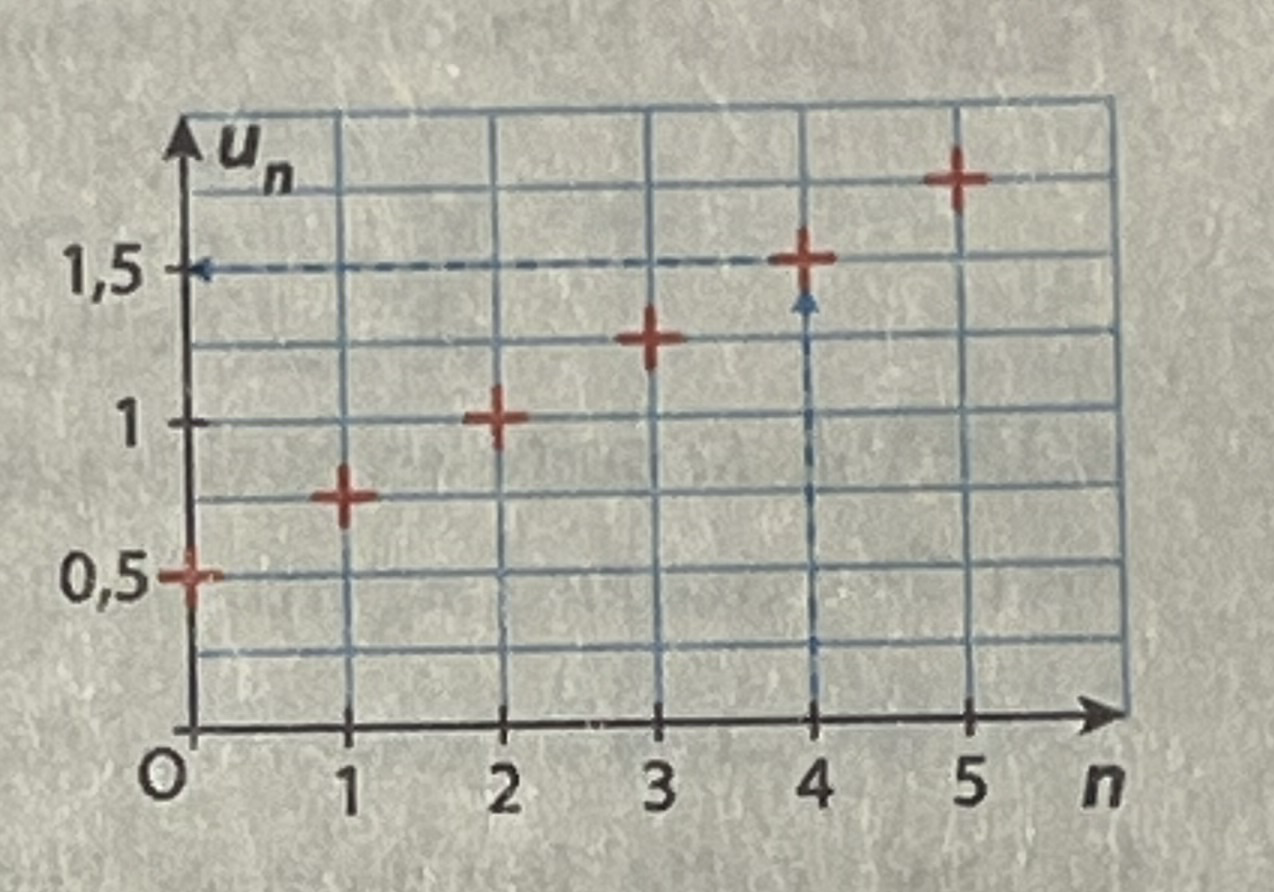
\includegraphics[scale=0.2]{1.OPT.02.03-Img01}

\begin{enumMet}
	\item Donner la valeur du 3ème terme de la suite. \corr{$u(2)=1$}
	\item Donner la valeur de $u(5)$. \corr{$u(5)=1,75$}
	\item Montrer que la suite $\left(u_n\right)$ est arithmétique et préciser sa raison et son premier terme.
	\begin{corrBox}
		Pour passer d'un terme au suivant on ajoute toujours 0,25. Il s'agit donc d'une suite arithmétique de raison 0,25 et de premier terme $u(0)=0,5$	
	\end{corrBox}
	\item En déduire le terme général de la suite.
	\begin{corrBox}
		terme général : $u(n)=u(0)+r\times n=0,5+0,25n$
	\end{corrBox}
	\item Donner la valeur du 25ème terme de la suite. \corr{$u(24)=0,5+0,25\times 24=6,5$}
\end{enumMet}

\end{document}

